\section{Generalising to 8-Connected Grid Maps}
Successfully applying Algorithm \ref{alg:rsr} to 8-connected grid maps 
involves adding a set of macro-edges between selected pairs of 
tiles on the perimeter of each empty rectangular room. 
We outline this process in two steps: 
\par
In the first step (Figure \ref{fig-macroedges} top), we add a series of macro 
edges between pairs of perimeter tiles on orthogonal sides of $R$. 
We connect two tiles only if the proposed macro edge represents a path through the interior of $R$ that involves
only diagonal transitions. Notice that this operation maintains the branching factor low.
It introduces no more than two macro-edges per tile.
\par
In the second step (Figure \ref{fig-macroedges} bottom), we add a series of macro 
edges between pairs of perimeter tiles on opposite sides of $R$.
We connect two tiles only if the proposed macro edge represents a path through the interior of $R$ which is shorter
than any alternative path involving only tiles from the perimeter and possibly one (other) macro edge.
For a perimeter tile such as $t_1$ we generate a ``fan'' of neighbours on the opposite side. The end tile $t_2$
in the fan is placed diagonally with respect to $t_1$. There is no need to add a macro-edge between $t_1$
and nodes beyond $t_2$ (e.g., $t_3$). Tile $t_3$ can be reached optimally from $t_1$ via the path
$\lbrace t_1, t_2, t_3 \rbrace$.

\begin{figure}[tb]
       \begin{center}
                       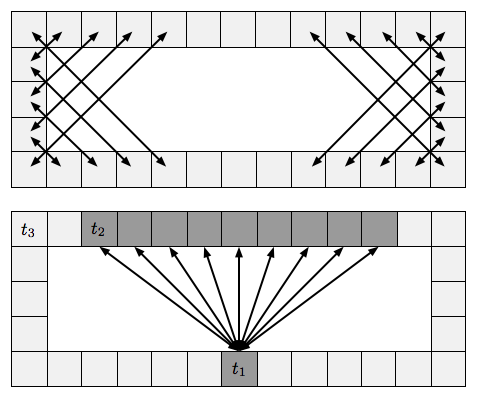
\includegraphics[scale=0.5, trim = 10mm 10mm 10mm 0mm]{diagrams/macroedges.png}
       \end{center}
	\vspace{-3pt}
       \caption{(Top) Macro edges between tiles on orthogonal sides of an empty room. 
(Bottom) Each tile on the perimeter is connected to a set of tiles on the opposite side of the room.}
       \label{fig-macroedges}
\end{figure}
We claim this method preserves optimality when traversing arbitrary rooms in an 8-connected grid map.
\begin{lemma}
\label{lemma-rooms}
Let $R$ be an empty rectangular room in an 8-connected grid map.
Further, let $m$ and $n$ be two locations along its perimeter.
Then, $m$ and $n$ can be connected optimally through a path that mentions only nodes on the perimeter of $R$ and
possibly involves one macro edge.
\end{lemma}

\begin{proof}
There are three cases to consider:
\begin{enumerate}
\item{$m$ and $n$ are on the same side of the perimeter.}
\item{$m$ and $n$ are on orthogonal sides of the perimeter.}
\item{\label{lemma-rooms-step3} $m$ and $n$ are on opposite sides of the perimeter.}
\end{enumerate}
In the first case we can simply walk along the perimeter from $m$ to $n$; the optimality of this path is immediate. 
In the second and third case we argue as follows: if $m$ and $n$ are not connected by a macro edge
we can walk along the perimeter from $m$ to the first intermediate node $m'$
which has a macro-edge incident with $n$. 
Since $m'$ is the first such node, the weight of the macro-edge $(m', n)$ is equal to
the diagonal distance between $m'$ and $n$. 
It is now easy to show that the length of the resultant path ${m, m', n}$ is equal to the octile distance between 
$m$ and $n$ and therefore optimal.
\end{proof}

\noindent
\textbf{Node Insertion:}
It is often the case that a tile from the interior of an empty room is required as a start or goal location for an
agent. 
To handle such situations we give an online procedure that temporarily re-inserts tiles back into the map for the duration
of a search. 
Our method is an adaptation of \citeauthor{harabor10}'s re-insertion algorithm
that specifically deals with 8-connected grids.
It proceeds as follows:

\begin{enumerate}
\item{If the start and goal are interior nodes in the same room no insertion is necessary; an optimal
path is trivially available. }
\item{If the start and goal are not in the same room, add four ``fans'' (collections) of macro edges.
Each fan connects the start (target) node to a set of nodes on one side of the room's perimeter.
The procedure is very similar to step 2 in the offline procedure: the fan should not go beyond tiles
placed diagonally with respect to the start (goal) tile at hand.}
\end{enumerate}
In an efficient implementation it is possible to identify in constant time the set of tiles which 
the start or goal must be connected to.
Further, these neighbours could be generated on the fly.
This means the time complexity associated with insertion can be as low as $O(1)$.
\begin{lemma}
\label{lemma-insertion}
Let $R$ be an empty rectangular room in an 8-connected grid map.
For any nodes $m$, $n$, with $m$ a re-inserted interior node and $n$ a node on the perimeter, it is always possible to
find an optimal length path which mentions no interior nodes except for $m$.
\end{lemma}
\begin{proof}
Our re-insertion procedure connects the start or goal to a set of nodes on each side of $R$.
The procedure in each case is the same as the one given when connecting two nodes on opposite sides of $R$.
To prove optimality we can simply run the argument given for Step \ref{lemma-rooms-step3} of Lemma \ref{lemma-rooms} for each
node on the perimeter of $R$, in each case substituting $m$ for the newly inserted node.
\end{proof}

%We claim that using the temporary macro edges added by this algorithm it is possible to travel optimally from the start or goal 
%location to any tile on the perimeter of the start or goal room. 
%\par \noindent
%\newline
We claim that the symmetry elimination procedure outlined in this section does not affect the optimality of solutions:
\begin{theorem}
For every optimal path $\pi$ on an original grid, there exists an optimal path $\pi'$ on the modfied graph with the property
that $\pi$ and $\pi'$ have the same cost.
\end{theorem}
\begin{proof}
Consider an optimal path $\pi$ on the original map and a room $R$ that is crossed by $\pi$.
Let $m$ and $n$ be the two perimeter points along $\pi$. According to Lemma~\ref{lemma-rooms},
there is a way to connect $m$ and $n$ optimally in the modified graph. Thus, we can replace the
original segment $[m \dots n]$ in $\pi$ with the cost-wise equivalent segment that corresponds to the modified graph.
The case when $m$ (or $n$) is the start or target node is addressed similarly using Lemma~\ref{lemma-insertion}.
By performing such a path segment replacement for all rooms intersected by $\pi$, we obtain a path $\pi'$
that satisfies the desired properties.
\end{proof}

%\textbf{Optimality:} We claim the symmetry elimination procedure outlined in this section is sufficient to guarantee
%that A*, running on a modified 8-connected grid map, will always find an optimal length solution if one exists.
%Our argument follows from Lemma \ref{lemma-rooms} and Lemma \ref{lemma-insertion}.
%It is based on the observation that for every segment of an optimal length path, which enters a room at some tile $m$,
%traverses through the interior of the room and exits at some tile $n$, there is an equivalent length path that mentions only 
%nodes from the perimeter of that room and possibly one macro edge.

